\chapter{Joshua 1}

\begin{figure}
  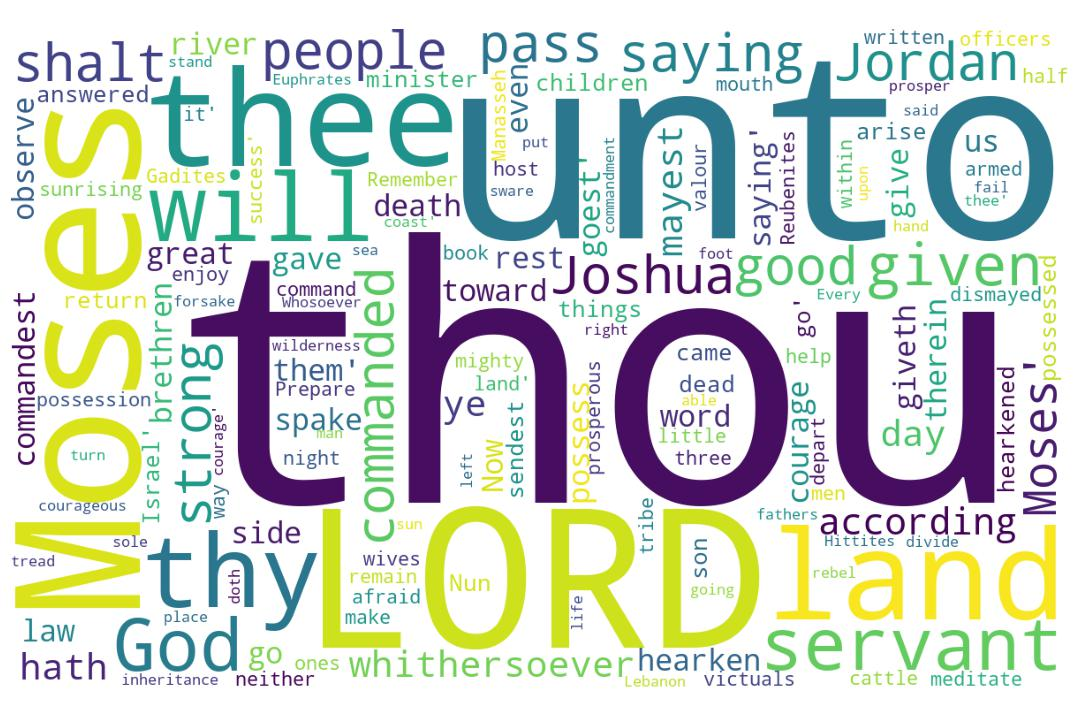
\includegraphics[width=\linewidth]{06OT-Joshua/Joshua1-WordCloud.jpg}
  \caption{Joshua 1 Word Cloud}
  \label{fig:Joshua 1 Word Cloud}
\end{figure}


\marginpar{\scriptsize \centering \fcolorbox{bone}{lime}{\textbf{NEW LEADER, WAITING LAND}}\\ (Joshua 1:1-18) \begin{compactenum}[I.][8]
    \item A \textbf{Son and his Legacy} \index[scripture]{Joshua!Jsh 01:01}(Jsh 1:1)
    \item A \textbf{Servant of the Lord} \index[scripture]{Joshua!Jsh 01:01}\index[scripture]{Joshua!Jsh 01:02}\index[scripture]{Joshua!Jsh 01:07}\index[scripture]{Joshua!Jsh 01:13}\index[scripture]{Joshua!Jsh 01:15}  (Jsh 1:1, 2, 7, 13, 15)
    \item Joshua \textbf{Assured for Life} \index[scripture]{Joshua!Jsh 01:05}(Jsh 1:5)
    \item  \textbf{Strength from the Law}  \index[scripture]{Joshua!Jsh 01:07}(Jsh 1:7)
    \item  \textbf{Success Limited} by adherence to the Law \index[scripture]{Joshua!Jsh 01:08}(Jsh 1:8)
    \item  \textbf{Sayings of a Leader} \index[scripture]{Joshua!Jsh 01:10} \index[scripture]{Joshua!Jsh 01:11}\index[scripture]{Joshua!Jsh 01:12}\index[scripture]{Joshua!Jsh 01:13}\index[scripture]{Joshua!Jsh 01:15} (Jsh 1:10, 11, 12, 13, 15)
    \item \textbf{Send us Into the Land!} \index[scripture]{Joshua!Jsh 01:16}(Jsh 1:16)
\end{compactenum}}

\footnote{\textcolor[cmyk]{0.99998,1,0,0}{\hyperlink{TOC}{Return to end of Table of Contents.}}}\footnote{\href{https://audiobible.com/bible/joshua_1.html}{\textcolor[cmyk]{0.99998,1,0,0}{Joshua Audio}}}\textcolor[cmyk]{0.99998,1,0,0}{Now after the death of Moses the \fcolorbox{bone}{lime}{servant of the LORD} it came to pass, that the LORD spake unto Joshua the \fcolorbox{bone}{lime}{son of Nun}, Moses' minister, saying,}
[2] \textcolor[cmyk]{0.99998,1,0,0}{Moses my \fcolorbox{bone}{lime}{servant} is dead; now therefore arise, go over this Jordan, thou, and all this people, unto the land which I do give to them, \emph{even} to the children of Israel.}
[3] \textcolor[cmyk]{0.99998,1,0,0}{Every place that the sole of your foot shall tread upon, that have I given unto you, as I said unto Moses.}
[4] \textcolor[cmyk]{0.99998,1,0,0}{From the wilderness and this Lebanon even unto the great river, the river Euphrates, all the land of the Hittites, and unto the great sea toward the going down of the sun, shall be your coast.}
[5] \textcolor[cmyk]{0.99998,1,0,0}{There shall not any man be able to stand before thee all the days of thy life: as I was with Moses, \emph{so} I will be with thee: I \fcolorbox{bone}{lime}{will not fail thee}, nor forsake thee.}
[6] \textcolor[cmyk]{0.99998,1,0,0}{Be strong and of a good courage: for unto this people shalt thou divide for an inheritance the land, which I sware unto their fathers to give them.}
[7] \textcolor[cmyk]{0.99998,1,0,0}{Only be thou \fcolorbox{bone}{lime}{strong} and very courageous, that thou mayest observe to do according to all the law, which Moses my \fcolorbox{bone}{lime}{servant} commanded thee: turn not from it \emph{to} the right hand or \emph{to} the left, that thou mayest prosper ommanded me, that ye should do so in the land whither ye go to possess it.}
[8] \textcolor[cmyk]{0.99998,1,0,0}{This book of the law shall not depart out of thy mouth; but thou shalt meditate therein day and night, that thou mayest observe to do according to all that is written therein: for then thou shalt make thy way prosperous, and then thou shalt have good \fcolorbox{bone}{lime}{success}.}
[9] \textcolor[cmyk]{0.99998,1,0,0}{Have not I commanded thee? Be strong and of a good courage; be not afraid, neither be thou dismayed: for the LORD thy God \emph{is} with thee whithersoever thou goest.}\\
\\
\P \textcolor[cmyk]{0.99998,1,0,0}{Then Joshua commanded the officers of the people, \fcolorbox{bone}{lime}{saying},}
[11] \textcolor[cmyk]{0.99998,1,0,0}{Pass through the host, and command the people, saying, Prepare you victuals; for within three days ye shall pass over this Jordan, to go in to possess the land, which the LORD your God giveth you to possess it.}\\
\\
\P \textcolor[cmyk]{0.99998,1,0,0}{And to the Reubenites, and to the Gadites, and to half the tribe of Manasseh, spake Joshua, saying,}
[13] \textcolor[cmyk]{0.99998,1,0,0}{Remember the word which Moses the \fcolorbox{bone}{lime}{servant} of the LORD commanded you, saying, The LORD your God hath given you rest, and hath given you this land.}
[14] \textcolor[cmyk]{0.99998,1,0,0}{Your wives, your little ones, and your cattle, shall remain in the land which Moses gave you on this side Jordan; but ye shall pass before your brethren armed, all the mighty men of valour, and help them;}
[15] \textcolor[cmyk]{0.99998,1,0,0}{Until the LORD have given your brethren rest, as \emph{he} \emph{hath} \emph{given} you, and they also have possessed the land which the LORD your God giveth them: then ye shall \fcolorbox{bone}{lime}{return} unto the land of your possession, and enjoy it, which Moses the LORD'S \fcolorbox{bone}{lime}{servant} gave you on this side Jordan toward the sunrising.}\\
\\
\P \textcolor[cmyk]{0.99998,1,0,0}{And they answered Joshua, saying, All that thou commandest us we will do, and whithersoever thou sendest us, we will go.}
[17] \textcolor[cmyk]{0.99998,1,0,0}{According as we hearkened unto Moses in all things, so will we hearken unto thee: only the LORD thy God be with thee, as he was with Moses.}
[18] \textcolor[cmyk]{0.99998,1,0,0}{Whosoever \emph{he} \emph{be} that doth rebel against thy commandment, and will not hearken unto thy words in all that thou commandest him, he shall be put to death: only be strong and of a good courage.}

